\documentclass[a4paper,12pt]{article} % тип документа

% report, book



%  Русский язык

\usepackage[T2A]{fontenc}			% кодировка
\usepackage[utf8]{inputenc}			% кодировка исходного текста
\usepackage[english,russian]{babel}	% локализация и переносы
\usepackage{graphicx}
\usepackage{tikz}
\graphicspath{{./}}
\DeclareGraphicsExtensions{.png,.jpg}


% Математика
\usepackage{amsmath,amsfonts,amssymb,amsthm,mathtools} 


\usepackage{wasysym}

%Заговолок
\author{Бредихин Александр}
\title{Домашняя работа №6}



\begin{document} % начало документа
\maketitle

\subsection*{Задача 1}

Подбрасываем <<честную>> монету $10$ раз. Подсчитайте вероятности следующих событий:

($i$) (1/6 балла)  число выпавших <<орлов>>  равно числу <<решек>>;\\

\textit{Решение:} используем схему Бернулли: так как количество выпадений орлов и решек совпадает, то 5 раз выпал орёл, 5 раз решка, получается:
$$
C_{10}^{5}\left(\frac{1}{2}\right)^{5}\left(\frac{1}{2}\right)^{5}=C_{10}^{5}\left(\frac{1}{2}\right)^{10}
$$

($ii$) (1/6 балла)  выпало больше <<орлов>>  чем <<решек>>;\\

\textit{Решение:} аналогично используем схему Бернулли: так как орлов выпало больше, чем решек, то возможны варианы -- 6 орлов, 7, 8, 9, 10. Для каждого применим схему Бернулли, получаем: 
$$
C_{10}^{6}\left(\frac{1}{2}\right)^{6}\left(\frac{1}{2}\right)^{4}+C_{10}^{7}\left(\frac{1}{2}\right)^{7}\left(\frac{1}{2}\right)^{3}+C_{10}^{8}\left(\frac{1}{2}\right)^{8}\left(\frac{1}{2}\right)^{2}+C_{10}^{9}\left(\frac{1}{2}\right)^{9}\left(\frac{1}{2}\right)^{1}+C_{10}^{10}\left(\frac{1}{2}\right)^{10}\left(\frac{1}{2}\right)^{0} =
$$
$$
= \left(\frac{1}{2}\right)^{10} \cdot \left(C_{10}^{6}+C_{10}^{7}+C_{10}^{8}+C_{10}^{9}+C_{10}^{10} \right) = 0.376953125
$$

($iii$) (1/6 балла) при $i=1,\dots,5$ одинаковы результаты $i$-го и $11-i$-го бросаний;\\

\textit{Решение:} Всего вариантов $ 2^{10} $ (на каждом из 10 бросков выпадает либо орёл, либо решка). Подходящих вариантов -- $ 2^5 $, так как при $i$-ом броске нас устраивают оба варианта, но для $11-i$-го броска задаётся одназначно (то что выпало на $i$-ом броске) $i=1,\dots,5 \longrightarrow 2^5$, тогда вероятность равна: 
$$
P = \frac{2^5}{2^{10}} = \frac{1}{2^5} = \frac{1}{32}
$$ 

($iv$) (1/2 балла) <<орел>> выпал не менее четырех раз подряд. \smallskip \\

\textit{Решение:} объединим 4 орла в 1 (чтобы гарантировать, что они всегда выпадут) и будем рассматривать как 7 элементов один из которых наш <<объединённый>> орёл. Разбиваем на случаи и считаем порядок с помощью формулы перестановок с повторениями сколько подходящих вариантов возможно. Пусть все оставшиеся выпали решки, тогда количество подходящих вариантов равно $ \frac{7!}{1! \cdot 6!} = 7 $. Если выпал ещё 1 орёл кроме заданных 4, тогда $ \frac{7!}{2! \cdot 5!} = 21 $ и так далее, последним будет вариант, когда выпали все орлы (только 1 комбинация). Подходящие варианты это сумма всех таких, их 127. Всего также $ 2^{10} $.\\
Ответ: 127/1024

\subsection*{Задача 2}
($i$) Вычислите условную вероятность, что при бросаний двух игральных костей на первой выпало шесть, если сумма равна семи.\\

\textit{Решение:}\\ Пусть: $ A $ -- событие: выпала сумма 7,\\
$ H_i $ -- гипотезы: выпало на 1ой кости $ i $,\\
тогда по формуле Байеса:
$$
P\left(H_{6} | A\right) = \frac{P\left(A | H_{6}\right) \cdot P\left(H_{6}\right)}{\sum\limits_{i=1}^{6} P\left(H_{i}\right) P\left(A | H_{i}\right)} = \frac{1 / 6^{2}}{6 \cdot 1 / 6^{2}}=1 / 6
$$
Ответ: 1 / 6\\

($ii$) При двух бросках игральной кости выпало $X_1$ и $X_2$, соответственно. Вычислите $\mathbb{E}\{\max\{X_1,X_2\}\} + \mathbb{E}\{\min\{X_1,X_2\}\}$.\\

Пусть $\xi = \max\{X_1,X_2\}$, а $ \eta =  \min\{X_1,X_2\}$. \\
По определению: $\mathbb{E}(\xi) = \sum\limits_{k=1}^{6} \xi \cdot P(\xi = k)$ и $ \mathbb{E}(\eta) = \sum\limits_{k=1}^{6} \eta \cdot P(\eta = k) $\\
Подсчитаем вероятности (подходящие варианты делим, на все: их всегда 36):\\
$ P(\xi = 1) = \frac{1}{36} = P(\eta = 6)$\\
$ P(\xi = 2) = \frac{3}{36} = P(\eta = 5)$\\
$ P(\xi = 3) = \frac{5}{36} = P(\eta = 4)$\\
$ P(\xi = 4) = \frac{7}{36} = P(\eta = 3)$\\
$ P(\xi = 5) = \frac{9}{36} = P(\eta = 2)$\\
$ P(\xi = 6) = \frac{11}{36} = P(\eta = 1)$\\
Получается, подставляя в формулы для мат. ожиданий $ \xi $ и $ \eta $ получаем:\\
$$\mathbb{E}(\xi) = \sum\limits_{k=1}^{6} \xi \cdot P(\xi = k) = \frac{1}{6^2} \cdot (1+6+15+28+45+66) = \frac{161}{36}$$
$$
\mathbb{E}(\eta) = \sum\limits_{k=1}^{6} \eta \cdot P(\eta = k) = \frac{1}{6^2} \cdot (11+18+21+20+15+6) = \frac{91}{36}
$$

$$
\mathbb{E}\{\max\{X_1,X_2\}\} + \mathbb{E}\{\min\{X_1,X_2\}\} = \mathbb{E}(\xi) + \mathbb{E}(\eta) = \frac{161}{36} + \frac{91}{36} = \frac{252}{36} = 7
$$
Ответ: 7

($iii$) Покажите, что из попарной независимости случайных величин не следует независимость в совокупности. Приведите контрпример.\\
Возьмём $ \Omega = \{ w_1, w_2, w_3, w_4\} $ и $ P(w_i) = 1/4 $\\
$ A = \{ w_1, w_2\}, B = \{ w_1, w_3\}, C = \{ w_1, w_4\} $\\

Заметим, что $ P(A) = P(B) = P(C) = \frac{1}{2} $\\
$ P(AB) = \frac{1}{4} = P(A) \cdot P(B)$, то есть попарная независимость\\
$ P(ABC) = \frac{1}{4} \neq P(A) \cdot P(B) \cdot P(C) = \frac{1}{8} $ -- нет независимости в совокупности.\\

($iv$) Независимы ли события: <<при броске кубика выпало четное число>> и <<при броске кубика выпало число, кратное трём>>?\\
$ A $ -- выпало чётное число. Подходят: 2 4 6 $ \Rightarrow P(A) = 1/2 $\\
$ B $ -- выпало число, кратное 3. Подходят: 3 6 $ \Rightarrow P(B) = 1/3 $\\
найдём $ P(AB) $: $ AB $ - чётное и кратное 3 $ \rightarrow $ только 6 $ \Rightarrow P(AB) = 1/6 $\\
Получается, что $ P(AB) = P(A) \cdot P(B) \Rightarrow \text{независимые}$\\

Ответ: независимые

($v$) Найти вероятность, что случайно выбранный граф на $n$ вершинах является простым циклом. Найти предел этой вероятности при $n\rightarrow \infty$. \\

В задача 5 подробно написано, что количество простых циклов на $ n $ вершинах равняется $ \frac{(n-1)!}{2} $ -- количество подходящих нам вариантов. Всего выриантов, то есть графов на $ n $ вершинах -- $ 2^{C_{n}^{2}} $ так как всего рёбер $ C_{n}^{2} $ и каждое из них мы можем брать или не брать. В итоге, по определению вероятности получаем ответ:\\

Ответ: $ \frac{(n-1)!}{2 \cdot 2^{C_{n}^{2}} } = \frac{(n-1)!}{2^{C_{n}^{2}+1} }$


\subsection*{Задача 3}
Две урны содержат одинаковое количество шаров. Шары окрашены в белый и черный цвета. Из каждой урны вынимают по $n$ шаров с возвращением, где $n \geq 3$. Найдите $n$ и <<состав>> каждой урны, если вероятность того, что все шары, взятые из первой урны, белые, равна вероятности того, что все шары, взятые из второй урны, либо белые, либо черные.\\

Так как мы возвращаем шары назад в урну каждый раз, когда достаём, то вероятность при следующем разе не изменится. Пусть всего в урнах $ x $ шаров и в первой урне $ a $ белых, а в правой $ b $ белых. Вероятность, что мы вытянем $ n $ раз белый шар из первой урны равна: $ \left(\frac{a}{x}\right)^n $. Вероятность вытянуть во второй урне все белые или все чёрные находим из формулы полной вероятности:\\
$ H_1 $ -1ым из второй урны вятянули белый, $ H_2 $ -- первым из второй урны вятянули чёрный, тогда $ P = \left(\frac{b}{x}\right)^n + \left(\frac{x-b}{x}\right)^n $. Из условия получаем, что:
$$
\left(\frac{a}{x}\right)^n = \left(\frac{b}{x}\right)^n + \left(\frac{x-b}{x}\right)^n
$$
Сократим на знаменатель в степени $ n $, получим:
$$
a^n = b^n + (x-b)^n
$$
Это выражение очень сильно похоже на великую теорему Ферма) \\
Это она и есть (так как по условию $ a $, $ b $, $ x $ целые числа). Но $n \geq 3$, поэтому по теореме решения в целых числах нет, следовательно, подходит только вариант, что $ x = b = a $ или $ b = 0, x = a $. То есть, что в первой урне лежат только белые шары, а в правой только чёрные или только белые. При этом $ n $ будет любым. Это и есть ответ.

\subsection*{Задача 4}
Симметричную монетку бросают неограниченное число раз. Какая из последовательностей встретится раньше с большей вероятностью: РОР или РРО? \\

Построим диграмму, как развивается игра (считаем, что один игрок ждёт РОР второй РРО)
\begin{center}
\begin{tikzpicture}[scale=0.2]
\tikzstyle{every node}+=[inner sep=0pt]
\draw [black] (16.8,-23.4) circle (3);
\draw (16.8,-23.4) node {$1$};
\draw [black] (31.1,-23.2) circle (3);
\draw (31.1,-23.2) node {$2$};
\draw [black] (45.7,-23.1) circle (3);
\draw (45.7,-23.1) node {$3$};
\draw [black] (45.7,-34.8) circle (3);
\draw (45.7,-34.8) node {$4$};
\draw [black] (61.1,-23.1) circle (3);
\draw (61.1,-23.1) node {$5$};
\draw [black] (61.1,-34.4) circle (3);
\draw (61.1,-34.4) node {$6$};
\draw [black] (19.8,-23.36) -- (28.1,-23.24);
\fill [black] (28.1,-23.24) -- (27.29,-22.75) -- (27.31,-23.75);
\draw (23.95,-23.81) node [below] {$P$};
\draw [black] (14.12,-24.723) arc (324:36:2.25);
\draw (9.55,-23.4) node [left] {$O$};
\fill [black] (14.12,-22.08) -- (13.77,-21.2) -- (13.18,-22.01);
\draw [black] (34.1,-23.18) -- (42.7,-23.12);
\fill [black] (42.7,-23.12) -- (41.9,-22.63) -- (41.9,-23.63);
\draw (38.4,-23.66) node [below] {$P$};
\draw [black] (44.104,-20.573) arc (240.00901:-47.99099:2.25);
\draw (44.78,-15.8) node [above] {$P$};
\fill [black] (46.73,-20.3) -- (47.57,-19.85) -- (46.7,-19.35);
\draw [black] (48.7,-23.1) -- (58.1,-23.1);
\fill [black] (58.1,-23.1) -- (57.3,-22.6) -- (57.3,-23.6);
\draw (53.4,-23.6) node [below] {$O$};
\draw [black] (33.45,-25.07) -- (43.35,-32.93);
\fill [black] (43.35,-32.93) -- (43.04,-32.04) -- (42.41,-32.83);
\draw (37.17,-29.49) node [below] {$O$};
\draw [black] (42.845,-35.715) arc (-76.01437:-147.04049:22.747);
\fill [black] (18.26,-26.02) -- (18.28,-26.96) -- (19.12,-26.42);
\draw (27.84,-35.33) node [below] {$O$};
\draw [black] (48.7,-34.72) -- (58.1,-34.48);
\fill [black] (58.1,-34.48) -- (57.29,-34) -- (57.31,-35);
\draw (53.41,-35.13) node [below] {$P$};
\end{tikzpicture}
\end{center}

Понятно, как эта диаграмма построена (смотрим, куда ведут нас все исходы выпадения монет). Подсчитаем вероятность, того что окажется комбинация РРО (то есть, что игрок, который ждёт эту комбинацию выиграет игрока, который ждёт РОР). Заметим, что $ p_5 = 0 $ (уже победа первого игрока), а $ p_6 = 1 $ (он уже точно проиграл). Запишем систему уравнений на вероятность каждого состояния в этой схеме (используя формулу полной вероятности):
$$
\begin{aligned}
&p_{2}=\frac{1}{2} p_{3}+\frac{1}{2} p_{4}\\
&P_{3}=\frac{1}{2} P_{3}+\frac{1}{2} P_{5}\\
&P_{1}=\frac{1}{2} p_{1}+\frac{1}{2} p_{6}\\
&P_{1}=\frac{1}{2} p_{1}+\frac{1}{2} p_{2}
\end{aligned}
$$
Решаем эту систему уравнений и находим: $ p_3 = 1 $, $ p_4 = 1/3 $ а $ p_1 = p_2 = 2/3 $. Получается, что комбинация РРО выпадет с большей вероятностью.

\subsection*{Задача 5}
($i$) Найти мат. ожидание числа простых циклов длины $r$ в случайном графе на $n$ вершинах. Любое из $C_n^2$ рёбер генерируется независимо от других с вероятностью $p$.\\

\textit{Решение:} аналогично задаче про треугольники из семинара:\\
На каждые $ r $ вершин <<посадим наблюдателя>>, то есть введём индикатор $ \xi_i $, который равняется 1, если $ i $ый простой цикл есть и 0, если его нет.\\
Всего простых циклов длины $ r $ в графе на $ n $ вершинах: $ \alpha =  C_{n}^{r} \cdot \frac{(n - 1)!}{2} $. Так как $ C_{n}^{r} $ -- количество способов выбрать $ r $ вершин, $ \frac{(n - 1)!}{2} $ -- количество простых циклов на $ r $ вершинах (начинаем с какой-то затем можем выбрать любую из $ (n-1) $ соединить с ней, затем выбираем вершину из $ (n-2) $ и соединяем её из последней, делим на 2 так как считаем в 2 стороны).\\
$$\mathbb{E}(\xi) = \mathbb{E}\sum\limits_{k=1}^{\alpha} \xi_i = \sum\limits_{k=1}^{\alpha}\mathbb{E} \xi_i = \sum\limits_{k=1}^{\alpha} p^r = \alpha \cdot p^r
$$

Ответ: $ \alpha \cdot p^r $\\

($ii$) Найти мат. ожидание числа простых циклов длины $r$ в случайной перестановке $n$ элементов в предположении, что все перестановки $\pi \in S_n$ равновероятны. \smallskip \\

Задача сводится к тому, что у нас есть граф, в котором нужно найти мат. ожидание простых циклов длины $ r $ (соответствующих случайной перестановке) только теперь (в отличие от предыдущего пункта) эти простые циклы не должны пересекаться и так как все перестановки равновероятны, то $ p = C_{n}^{2} $. То что циклы не пересекаются учитываем тем, что на $ r $ вершинах нам подходит только один вариант. Поэтому ответ будет выглядить как $ \alpha \cdot p^r $, где $ \alpha = C_{n}^{r} $, а $ p = C_{n}^{2} $.

\subsection*{Задача 6}
Имеется генератор случайных битов, выдающий $0$ и $1$ с вероятностью $1/2$. Предложите алгоритм, использующий этот генератор и выдающий $0$ с вероятностью $1/3$ и $1$ с вероятностью $2/3$. Оцените матожидание времени работы алгоритма. \\

1) Запустим два раза генератор случайных чисел (равновероятный), получим 4 возможных равновероятных варианта (каждый с вероятностью 1/4):\\
\begin{tabular}{|c|c|c|}
\hline 
$x_1$ & $x_2$ & $P$ \\ 
\hline 
0 & 0 & 1/4 \\ 
\hline 
0 & 1 & 1/4 \\ 
\hline 
1 & 0 & 1/4 \\ 
\hline 
1 & 1 & 1/4 \\ 
\hline 
\end{tabular} 
\smallskip \\
Сделаем так: если выпадает 0 0, возвращаем 0, если выпадает 1 0 или 0 1, то возвращаем 1, если 1 1, то запускаем алгоритм заново. Получается, 0 выводится в 1 из 3 случаев, то есть $ P(0)=1/3 $, а 1 в 2 из 3 случаях, то есть $ P(1) = 2/3 $.\\
Реализайия этого алгоритма на Python ($rand\_eq$ - равновероятная функция)
\begin{center}
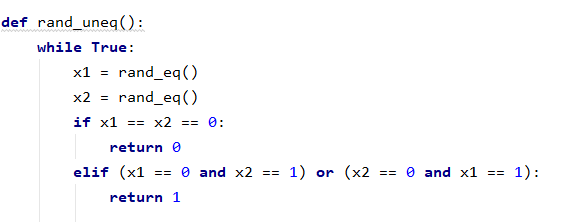
\includegraphics[width=0.7\textwidth]{code}
\end{center} 

Заметим, что алгоритм закончится, так как вероятность того, что мы начинаем цикл заново $ n $ раз равна: $ (1/4)^n \rightarrow 0 $ при $n\rightarrow \infty$\\

Мат. ожидание количества итераций находим по определению:
$$
\mathbb{E}\xi = \sum\limits_{k=1}^{\infty} k \cdot \left(\frac{1}{4}\right)^k = \frac{13}{9}
$$
(подсчитал численно)\\

2) Обратно делаем аналогично: запускаем наш генератор $rand\_uneq$ два раза, получаем такие случаи:
\begin{tabular}{|c|c|c|}
\hline 
$x_1$ & $x_2$ & $P$ \\ 
\hline 
0 & 0 & 1/9 \\ 
\hline 
0 & 1 & 2/9 \\ 
\hline 
1 & 0 & 2/9 \\ 
\hline 
1 & 1 & 4/9 \\ 
\hline 
\end{tabular} 
\smallskip \\
Заметим, что вероятность выпадения 1 1 и вероятность выпадения комбинаций 1 0 и 0 1 совпадает и равна 4/9, следовательно, будем выводить 1 (в 4 из 8 случаев вывода) при выпадении 1 1 и 0 при выпадении 1 0 или 0 1 (также в 4 из 8 случаев). Если выпадает 0 0, то запускаем заново. Получаем равновероятный генератор.\\
Этот алгоритм также закончится, так как вероятность того, что мы начинаем цикл заново $ n $ раз равна: $ (1/9)^n \rightarrow 0 $ при $n\rightarrow \infty$\\

Мат. ожидание количества итераций находим по определению:
$$
\mathbb{E}\xi = \sum\limits_{k=1}^{\infty} k \cdot \left(\frac{1}{9}\right)^k = \frac{73}{64}
$$
(подсчитал численно)

\subsection*{Задача 7}
Найти мат. ожидание количества неподвижных элементов в случайно выбранной из $S_n$ перестановке.  \smallskip \\

Пусть $ \xi $ -- случайная величина равная количеству неподвижных элементов в $S_n$ перестановке.\\
Введём индикатор $ \xi_i $:\\
$ \xi_i = 1 $ если в случайной перестановке $ x_i = i $\\
$ \xi_i = 0 $ иначе\\
$ \xi = \sum\limits_{i=1}^{n} \xi_i$\\
Пользуемся линейностью матожидания и тем, что $ \mathbb{E}(\xi) $ равны $\forall i = 1, \ldots, n$ (так как без разницы на какую позицию смотреть), получаем:
$$\mathbb{E}(\xi) = \mathbb{E}\sum\limits_{k=1}^{n} \xi_i = \sum\limits_{k=1}^{n}\mathbb{E} \xi_i = n \cdot \mathbb{E} \xi_1 = n \cdot P(\xi_1 = 1) = n \cdot P(x_1 = 1) = n \cdot \frac{(n-1)!}{n!} = n \cdot \frac{1}{n} = 1$$
Последние получается так, что мы ставим первый элемент на 1ое место (на его собственное) а остальные можно переставлять как угодно $ \longrightarrow $ $ (n-1)! $. А всего -- $ n! $\\
Ответ: 1

\subsection*{Задача 8}
В экзаменационной программе обычного экзамена $25$ билетов, из которых $5$ простые, а вытянув любой из остальных, всякий студент точно завалит экзамен. Подряд заходят два студента. Какой из них с большей вероятностью вытянет простой билет? (используйте для второго студента формулу полной вероятности для двух возможных результатов первого студента). \smallskip \\

Пусть $ A $ -- второй студент вытянет простой билет\\
Гипотезы: $ H_1 $ -- первый студент вытянет простой билет, $ H_2 $ -- первый студент вытянет сложный билет. По формуле полной вероятности:\\
$$
P(A) = P(H_1) \cdot P(A | H_1) + P(H_2) \cdot P(A | H_2) = \frac{5}{25} \cdot \frac{4}{24} + \frac{20}{25} \cdot \frac{5}{24} = \frac{20+100}{25 \cdot 24} = 1/5
$$
Заметим, что $ P(H_1) = \frac{5}{25} = 1/5 $\\
Следовательно оба студента вытянут простой билет с одинаковой вероятностью равной $ 1/5 $\\
Ответ: равновероятны, $ P(A) = 1/5 $



\subsection*{Задача 9}
Найти математическое ожидание числа бросаний кости до первого выпадения двух шестерок подряд. \smallskip \\

Введём две случайные величины: $ \xi $ -- количество бросаний до появления двух шестёрок подряд и $ \eta $ -- количество бросаний до появления двух шестёрок подряд при условии что только что выпала 6. Вероятность выпадения шестёрки при каждом бросании кубика равна - $ 1/6 $. Вероятность выпадения всего остального - $ 5/6 $.\\
Пользуясь идеей формулы полной вероятности (учитывая этот бросок) получим уравнения на мат. ожидания наших случайных величин. 
$$\begin{array}{c}
\mathbf{E}{\xi}=\frac{5}{6}\left(1+\mathbf{E}{\xi}\right)+\frac{1}{6}\left(1+\mathbf{E}{\eta}\right) \\
\mathbf{E}{\eta}=\frac{1}{6} \cdot 1+\frac{5}{6}\left(1+\mathbf{E}{\xi}\right)
\end{array}$$

Из второго уравнения находим, что $ \mathbf{E}{\eta}= 1+\frac{5}{6}\mathbf{E}{\xi} $, подставляем в первое и находим $ \mathbf{E}{\xi} = 42 $.\\
Ответ: 42


\subsection*{Задача 10}
На окружности случайным образом выбираются две точки. Найдите среднее расстояние между ними. \\

Понятно, что первую точку мы выбираем в произвольном месте окружности. Затем через эту выбранную точку мы можем провести касательную. Будем определять вторую точку, как угол между этой касательной и секущей. Из геометрии найдём, что угол и расстояние между точками связываются следующей формулой: $ \xi = D \cdot \sin\alpha $, где $ \xi $ -- случайная величина: расстояние между точками окружности. $ D $ - диаметр окружности. \\

Пользуясь линейностью мат. ожидания получаем $ \mathbf{E}{\xi} = D \cdot \mathbf{E}{\alpha} $\\
Мат ожидание угла из соображений найдём из того, что распределение точек на окружности равновероятно $ \longrightarrow $ распределение $ \alpha $ равномерно. Получается:
$$
\mathbf{E}{\xi} = D \cdot \mathbf{E}{\alpha} = \frac{D}{\pi} \int_{0}^{\pi} \sin \alpha d \alpha=\frac{2D}{\pi}
$$
Ответ: $ \frac{2D}{\pi} $
\end{document}

\end{document} % конец документа